%!TEX root = /Users/stevenmartell/Documents/CURRENT PROJECTS/iSCAM-trunk/fba/BC-herring-2011/WRITEUP/BCHerring2011.tex
\section{Methods}
	\subsection{Input data \& assumptions}
	\subsubsection{Catch data}
	For each of the statistical areas, the required input data for \iscam\ consists of a catch time series for each of the fishing fleets.  For the BC herring fishery, the annual total removals has been partitioned into three distinct fishing fleets (or fishing periods, see Figure \ref{FigCatch}).  The first fleet is a winter seine fishery that has been in operation since the start of the assessment in 1951, the second is a seine-roe fishery that commenced in 1972 in the Strait of Georgia, and the third fleet is a gillnet fishery that targets females on the spawning grounds. The model is fit to the catch time series information and assumes measurement errors are lognormal, independent and identically distributed.  The assumed standard deviation in the catch observations must be specified in the control file and it is assumed that measurement errors in the catch is the same for all fishing periods.  The units of the catch are given in 1000s of metric tons.
	
	In addition to the commercial catch, removals from fisheries independent surveys must also be specified in \iscam. Two additional fleets are specified to represent the spawn survey, where the spawn survey is broken into two distinct time periods pre-1988 and post-1988, the year when the survey switched from surface surveys to dive surveys.  This partitioning of the data is done for two reasons: (1) to allow for different catchability coefficients to be specified for the early and late periods, and to allow for more weight to be placed on the contemporary data due to improved precision in the estimates of egg layers. 

%TODO decide if the test fishery data is going to be looked at here or in the appendix
	In the case where the test fishery data has been separated from the seine roe fishery, an additional fleet is specified in the data file and fishing mortality rates for the test fishery are also estimated in years when the catch is greater than 0.
	
\begin{figure}[!tbp]
	% Requires \usepackage{graphicx}
	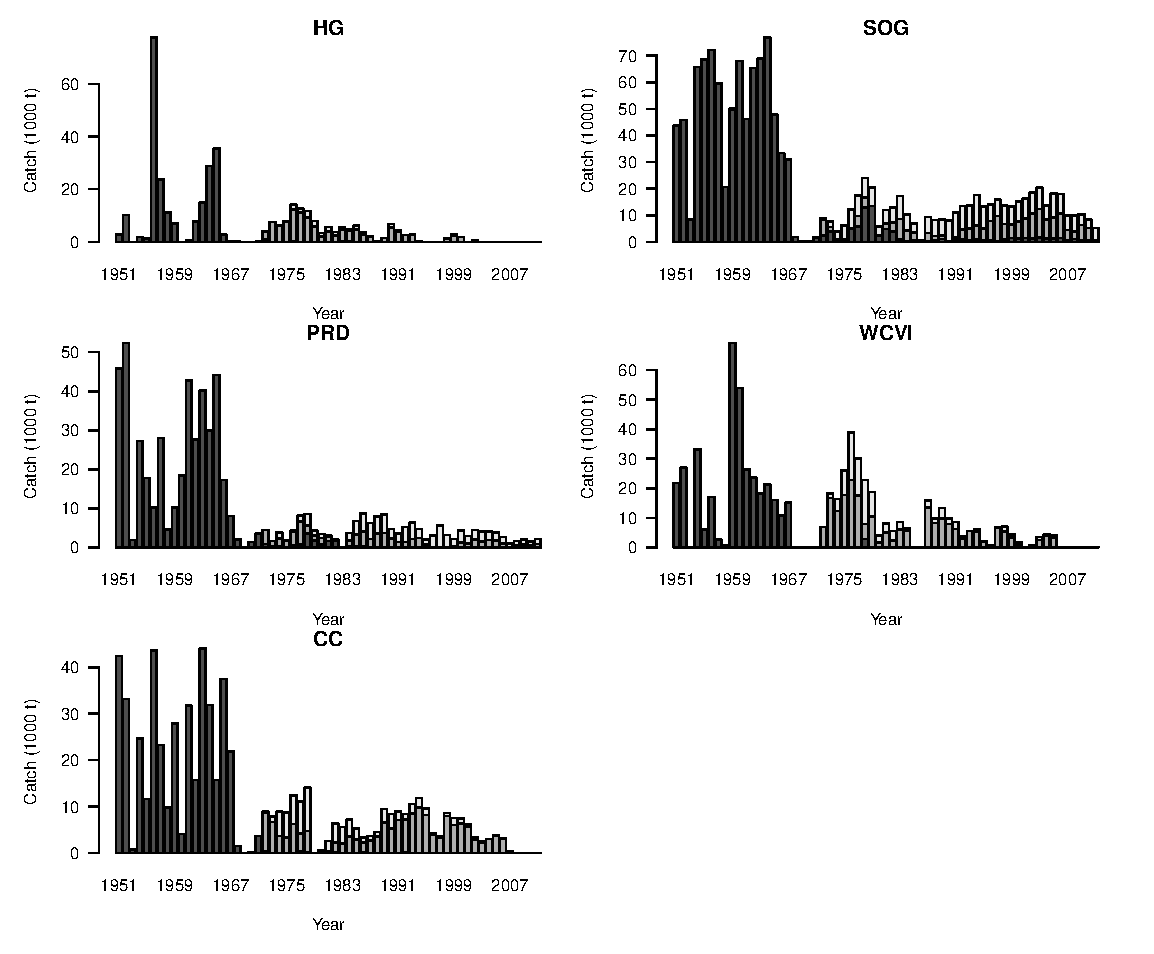
\includegraphics[width=\textwidth]{../Figs/iscam_fig_CatchMajorAreas.pdf}\\
	\caption{Historical catch of herring in the five major stock areas between 1951 and 2011 for the winter purse seine fishery (dark bars), seine-roe fishery (grey bars), and gill net fishery (light grey bars). Units of catch are in thousands of metric tons.}\label{FigCatch}
\end{figure}
	
	\subsubsection{Relative abundance data}
Herring spawn surveys have been conducted throughout the B.C. coast beginning in the 1930s. Prior to 1988, spawn surveys were conducted from the surface either by walking the beach at low tide or using a drag from a skiff to estimate the shoreline length and width of spawn. Egg layers were sampled visually and are used to calculate egg densities following the methods of Schweigert (2001). Beginning in 1988, herring spawn surveys using SCUBA methods were introduced and were implemented coastwide within a couple of years initially being conducted by DFO staff and eventually through contract divers hired through the test fishing program. Prior to the 2006 Larocque ruling, the test fishing program was funded through an allocation of fish by industry. In years since the 2006 Larocque ruling, the availability of resources to conduct dive surveys in all areas has been reduced. For the 2010 survey, dive surveys were conducted in all major and minor assessment regions, with the exception of Area 2W where snorkeling and surface survey methods were also used. As in earlier years, a few minor spawning beds outside the main assessment areas were surveyed by SCUBA or surface methods where resources permitted.


The locations of the spawning beds for the five major and two minor stock areas are shown in Figure \ref{figSpawnMaps}.  Egg density estimates are used to claculate a fishery-independent index of herring spawning biomass, referred to as the spawn survey index hereafter \citep{schweigert2001stock}.

\begin{figure}[!tbp]
	% Requires \usepackage{graphicx}
	\centering
	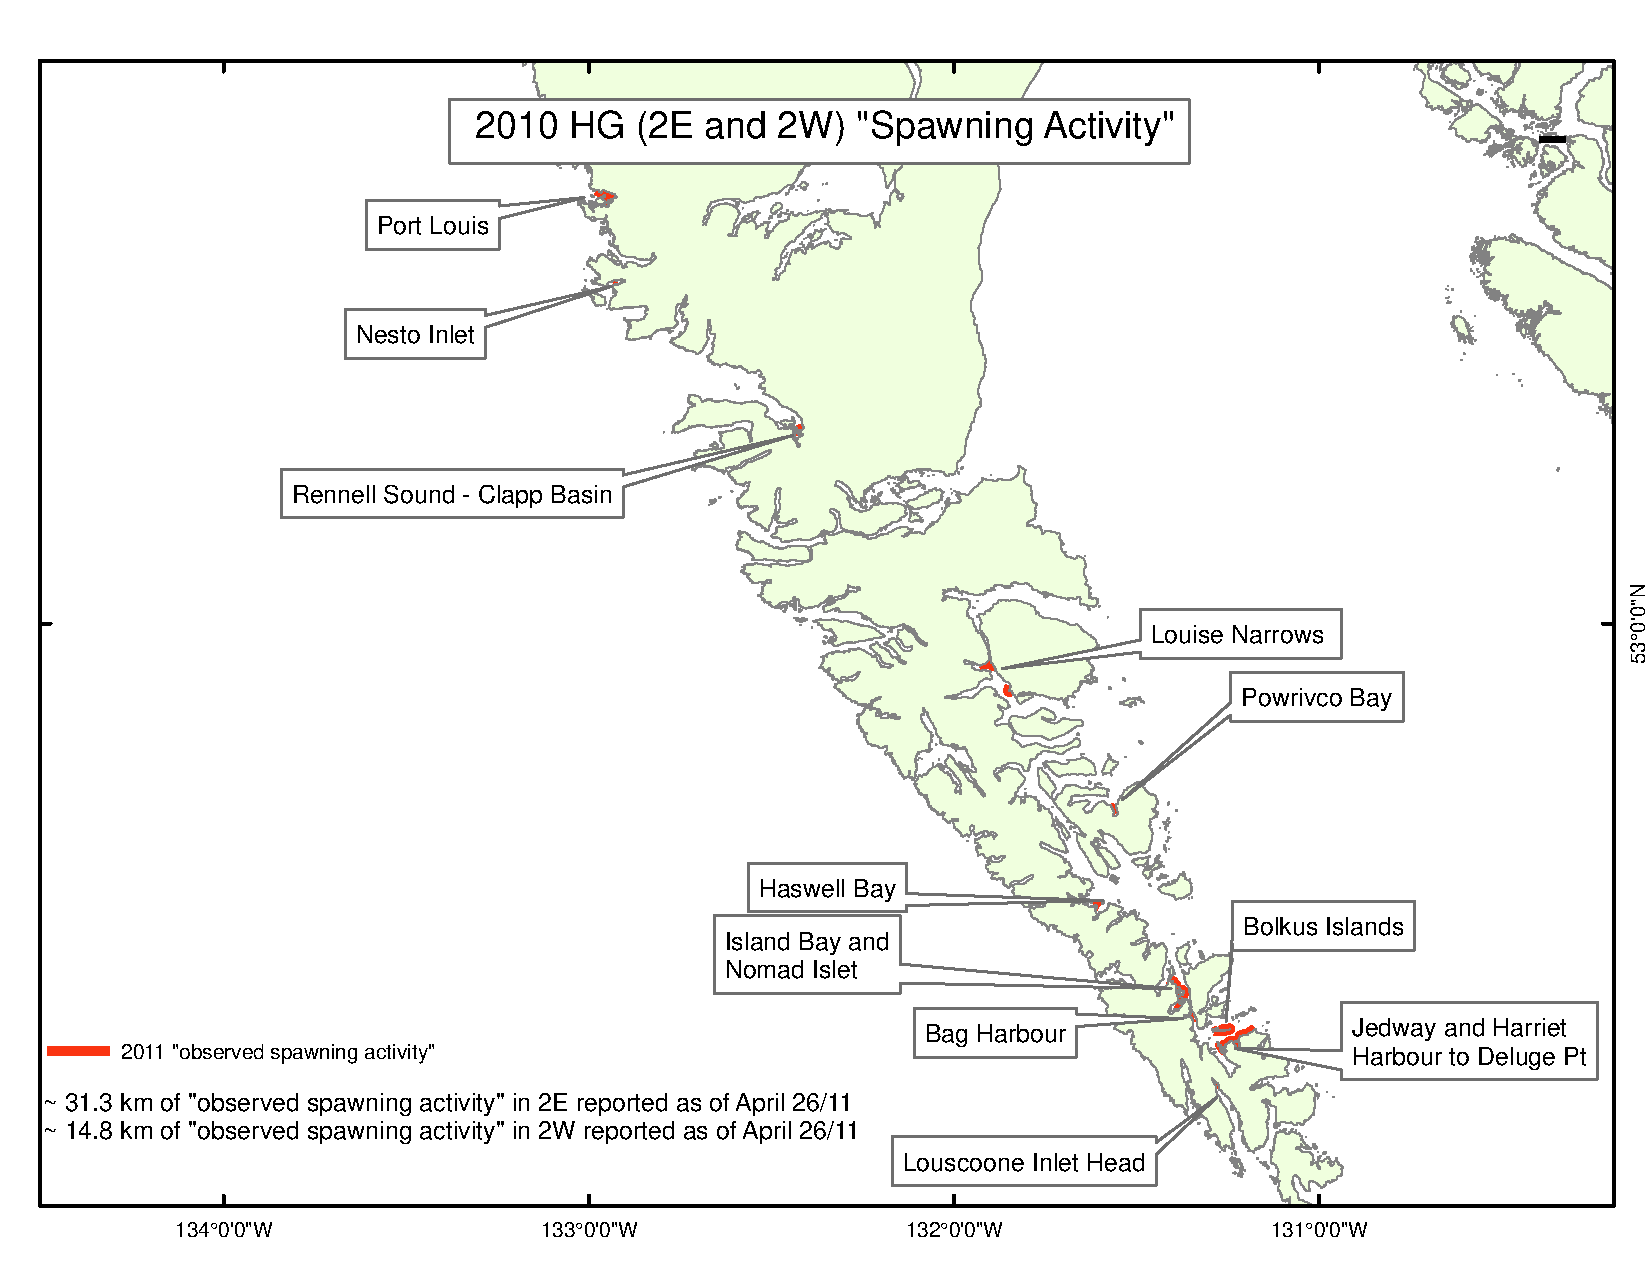
\includegraphics[scale=0.5]{../Figs/PBSfigs/2011-HG-Prelim-WG.pdf}\\
	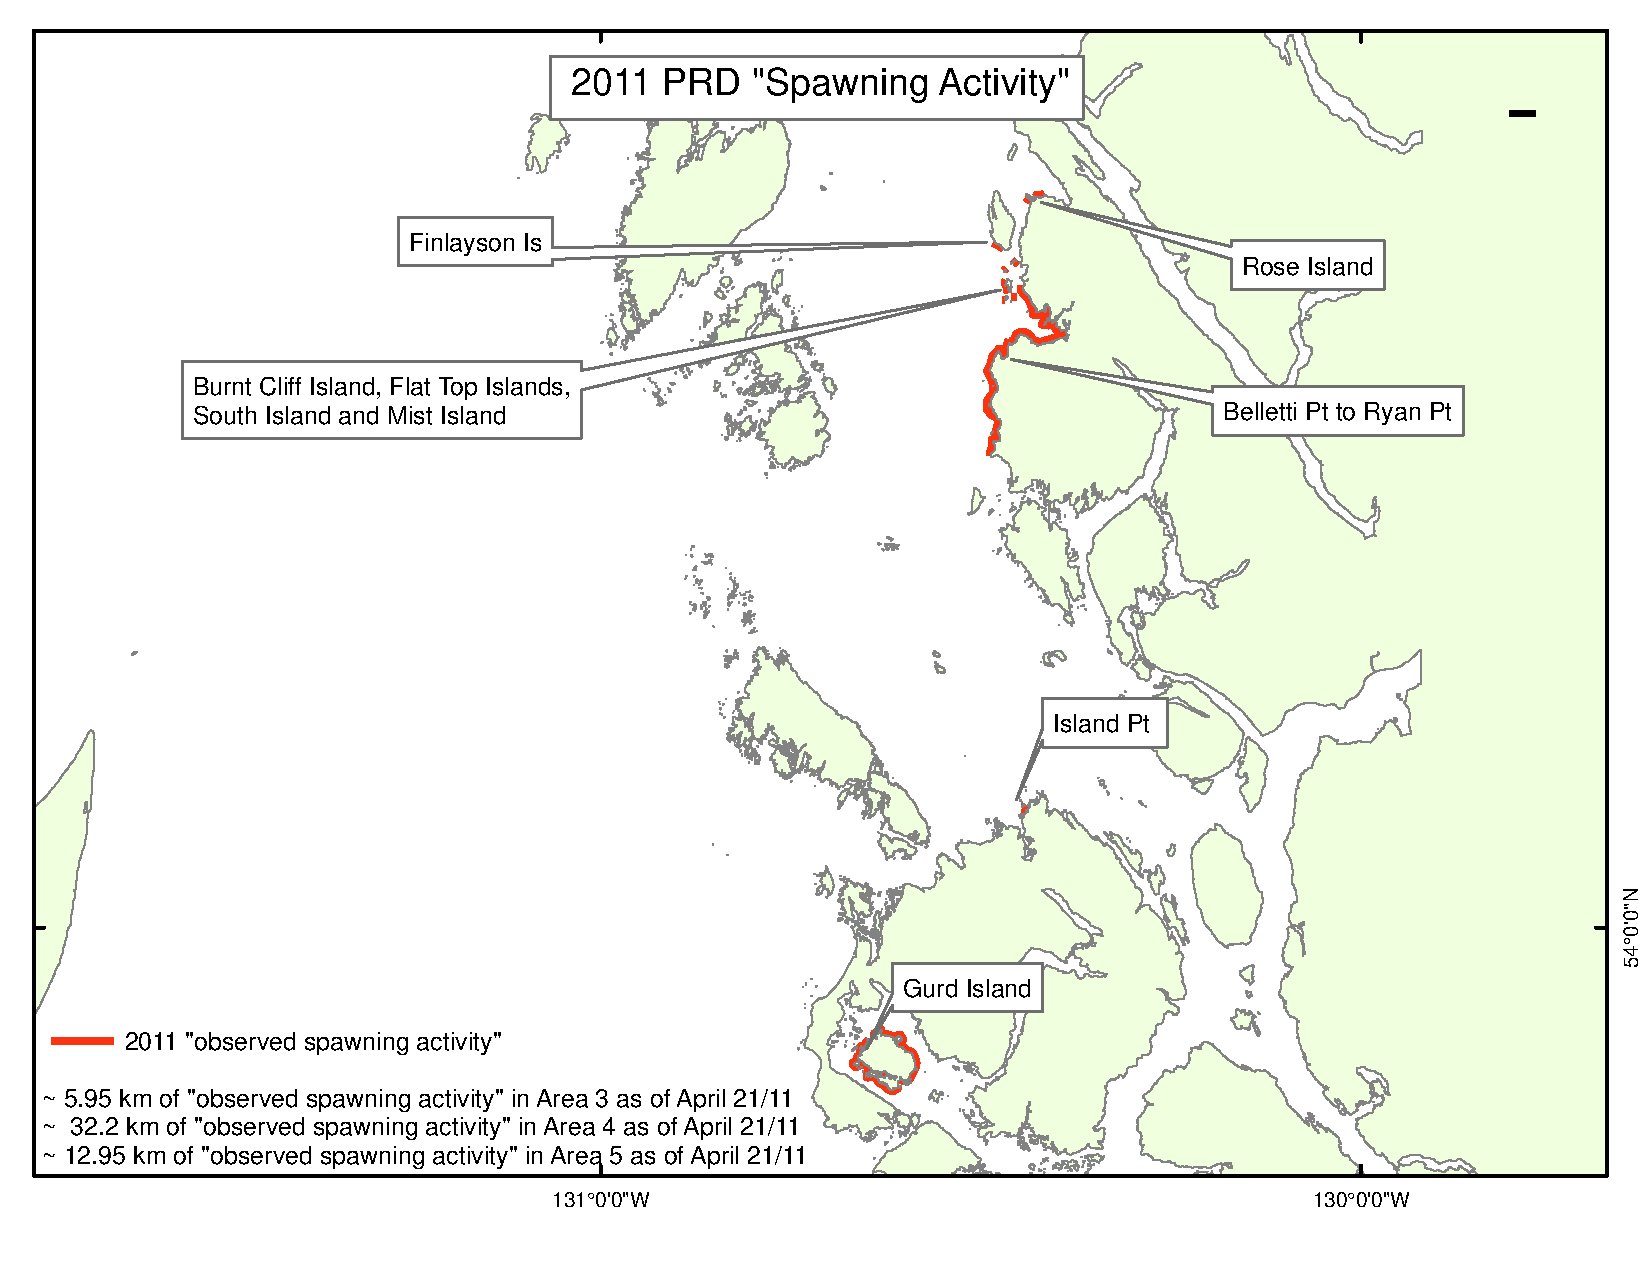
\includegraphics[scale=0.5]{../Figs/PBSfigs/2011-PRD-Prelim-WG.pdf}
	\caption{Preliminary Spawning activity for Haida Gwaii (top panel) and Prince Rupert District (bottom) in 2011.}
\end{figure}
\begin{figure}[!tbp]
	% Requires \usepackage{graphicx}
	\ContinuedFloat
	\centering
	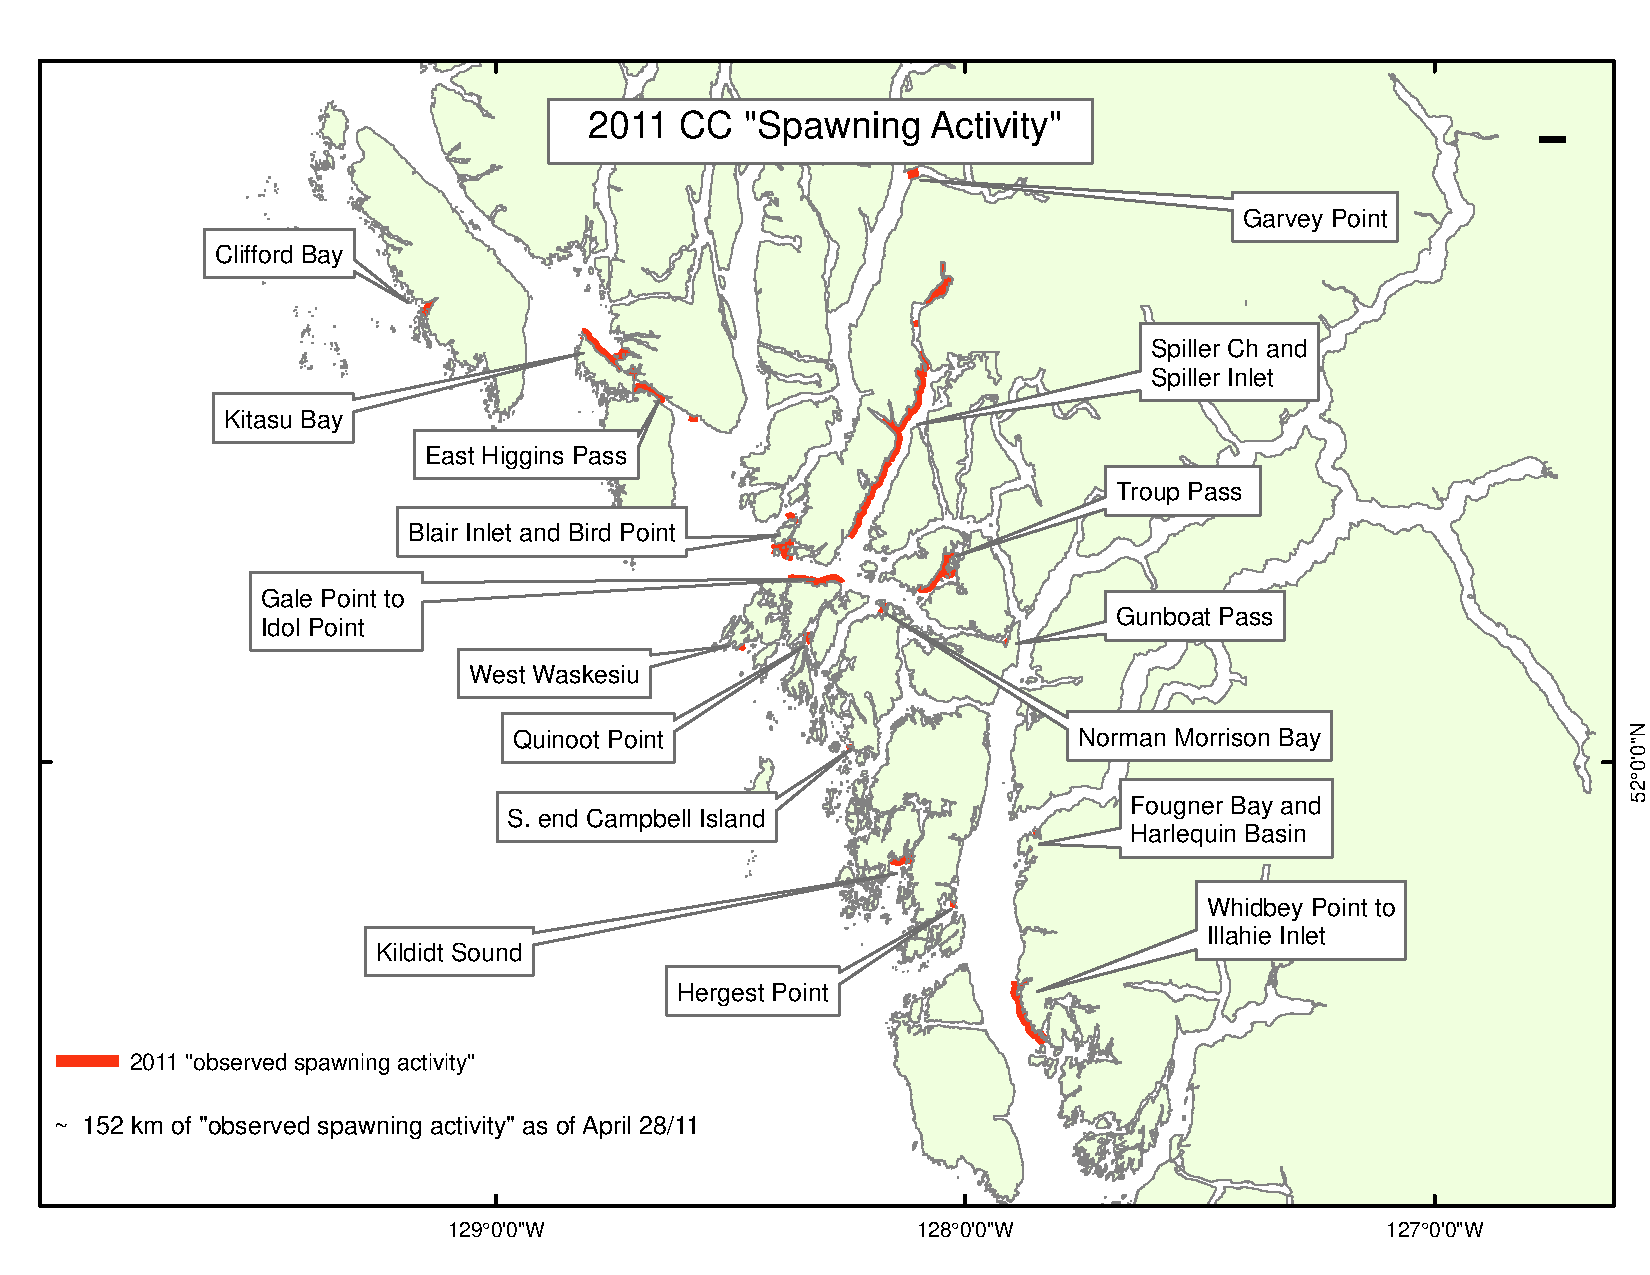
\includegraphics[scale=0.5]{../Figs/PBSfigs/2011-CC-Prelim-WG.pdf}\\
	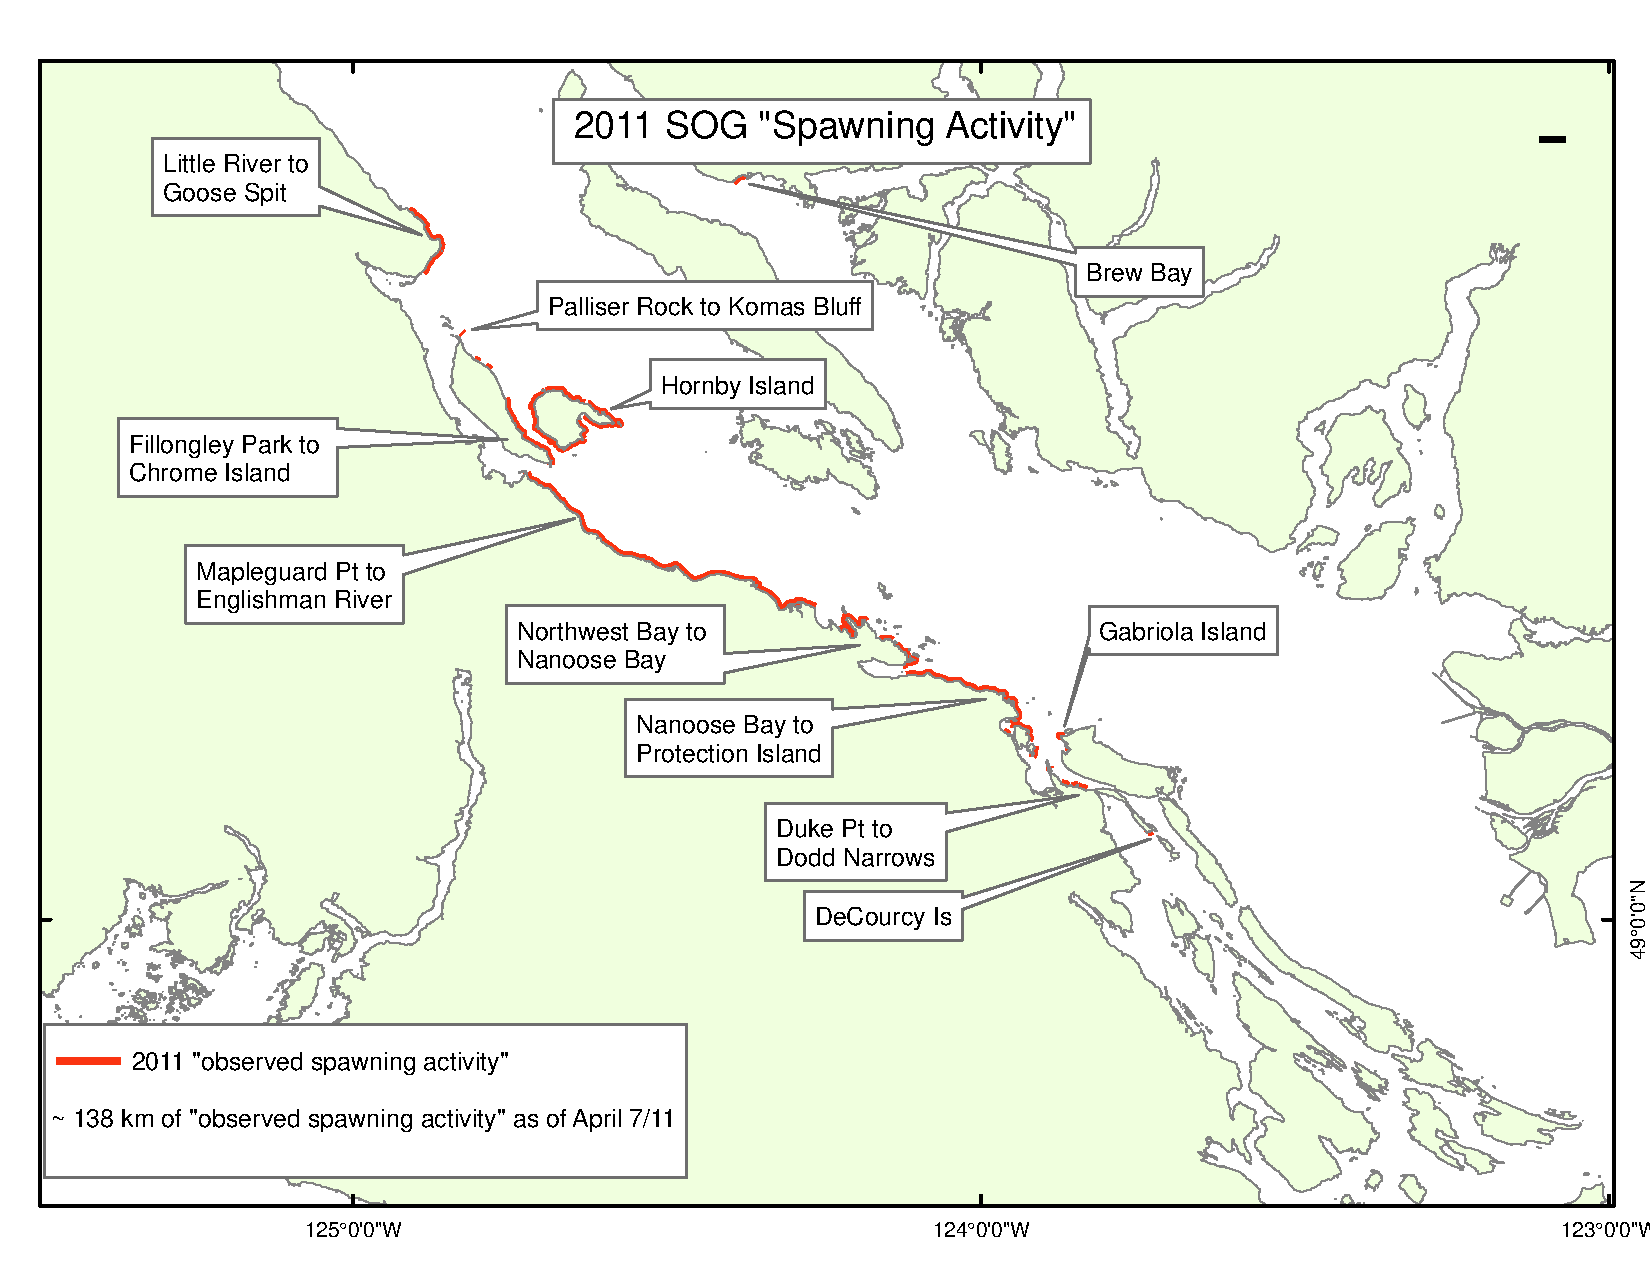
\includegraphics[scale=0.5]{../Figs/PBSfigs/2011-SOG-Prelim-WG.pdf}
	\caption{Preliminary Spawning activity for Central Coast (top panel) and Strait of Georgia (bottom) in 2011.}
\end{figure}
\begin{figure}[!tbp]
	% Requires \usepackage{graphicx}
	\ContinuedFloat
	\centering
	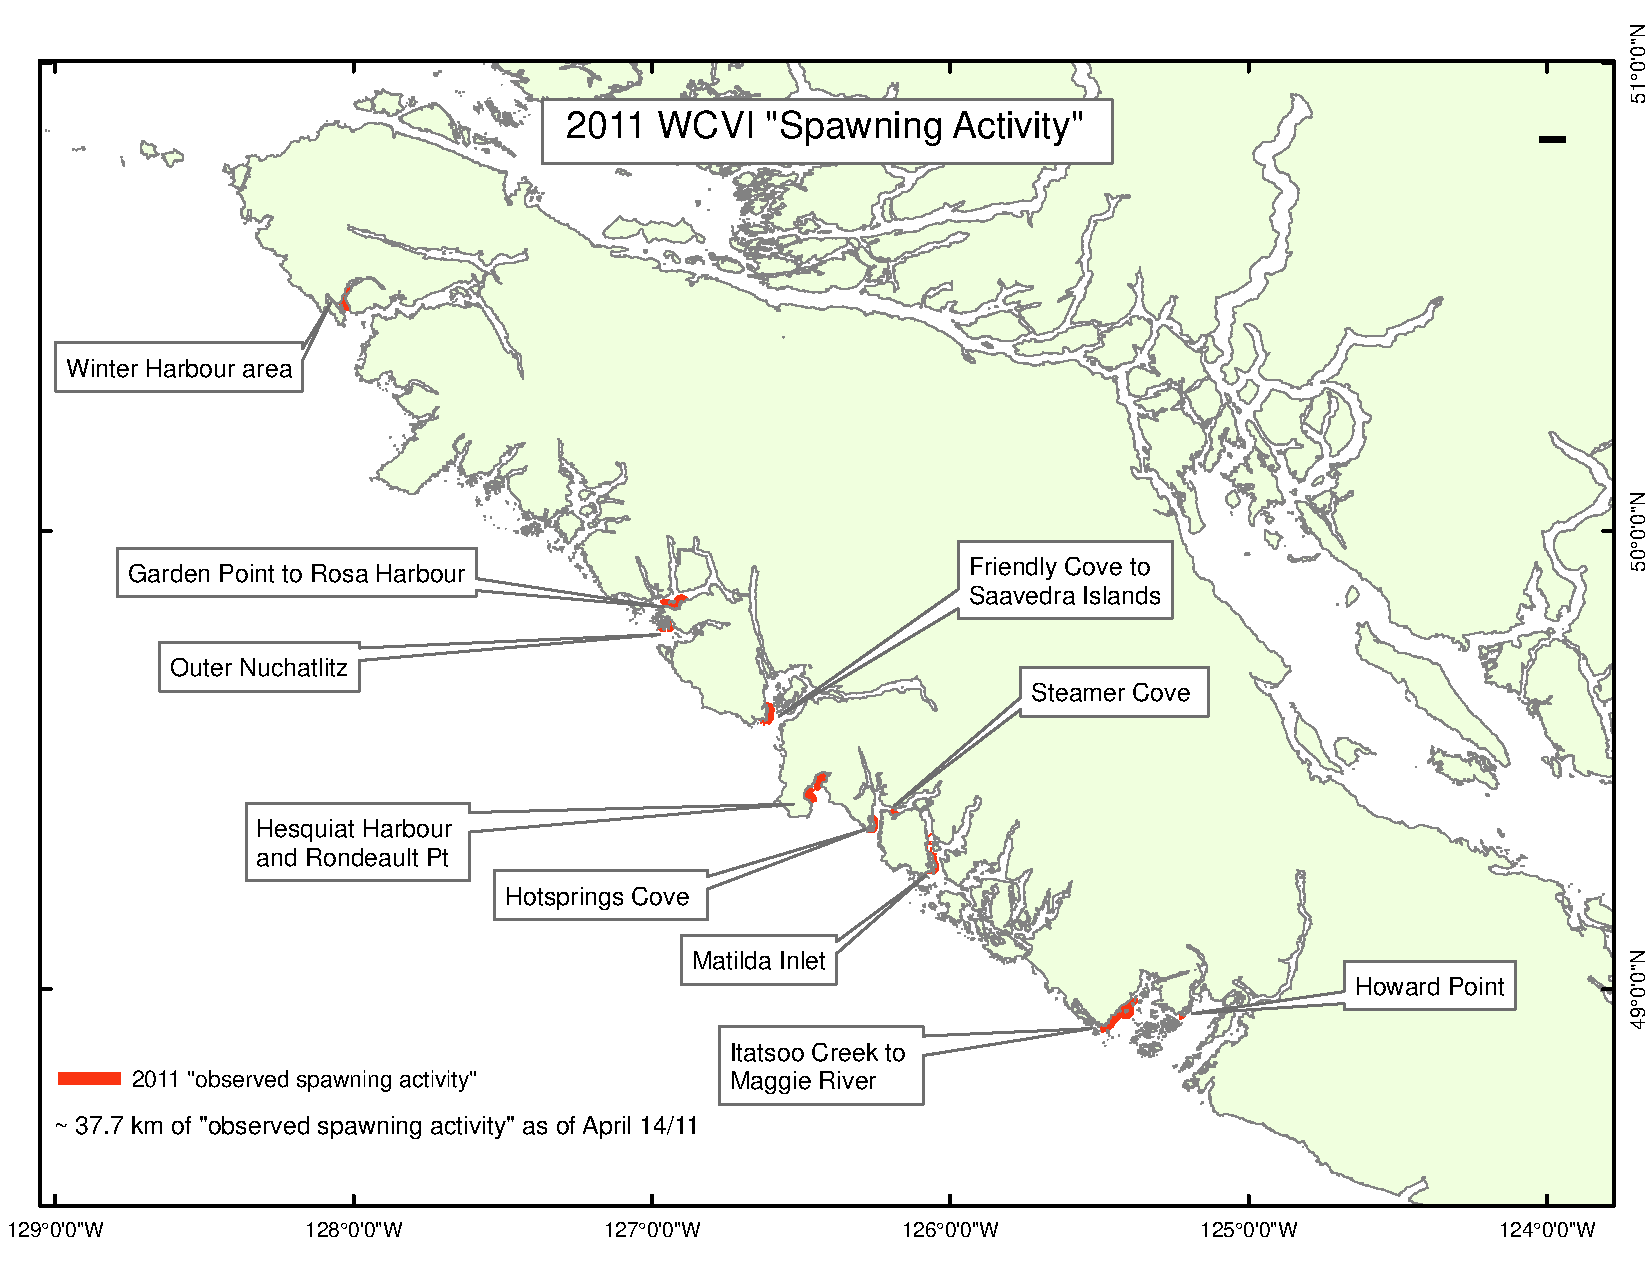
\includegraphics[scale=0.5]{../Figs/PBSfigs/2011-WCVI-Prelim-WG.pdf}\\
	\caption{Preliminary Spawning activity in 2011 for the West Coast of Vancouver Island (includes minor stock area 27).}\label{figSpawnMaps}
\end{figure}

	The spawn survey is conducted after the fisheries in the area have been conducted; therefore, it is assumed that all the mortality for the year has occurred just prior to commencing the spawning survey. The fisheries independent survey estimates egg density and total spawn area, and from this information the total female spawning biomass can be estimated assuming the 227 eggs per gram of female  or 114 eggs per gram of mature spawning individuals \citep{hardwick1973biomass}. The assumed selectivity for the spawn survey is fixed to the maturity schedule for herring.  	
	
\begin{figure}[!tbp]
	% Requires \usepackage{graphicx}
	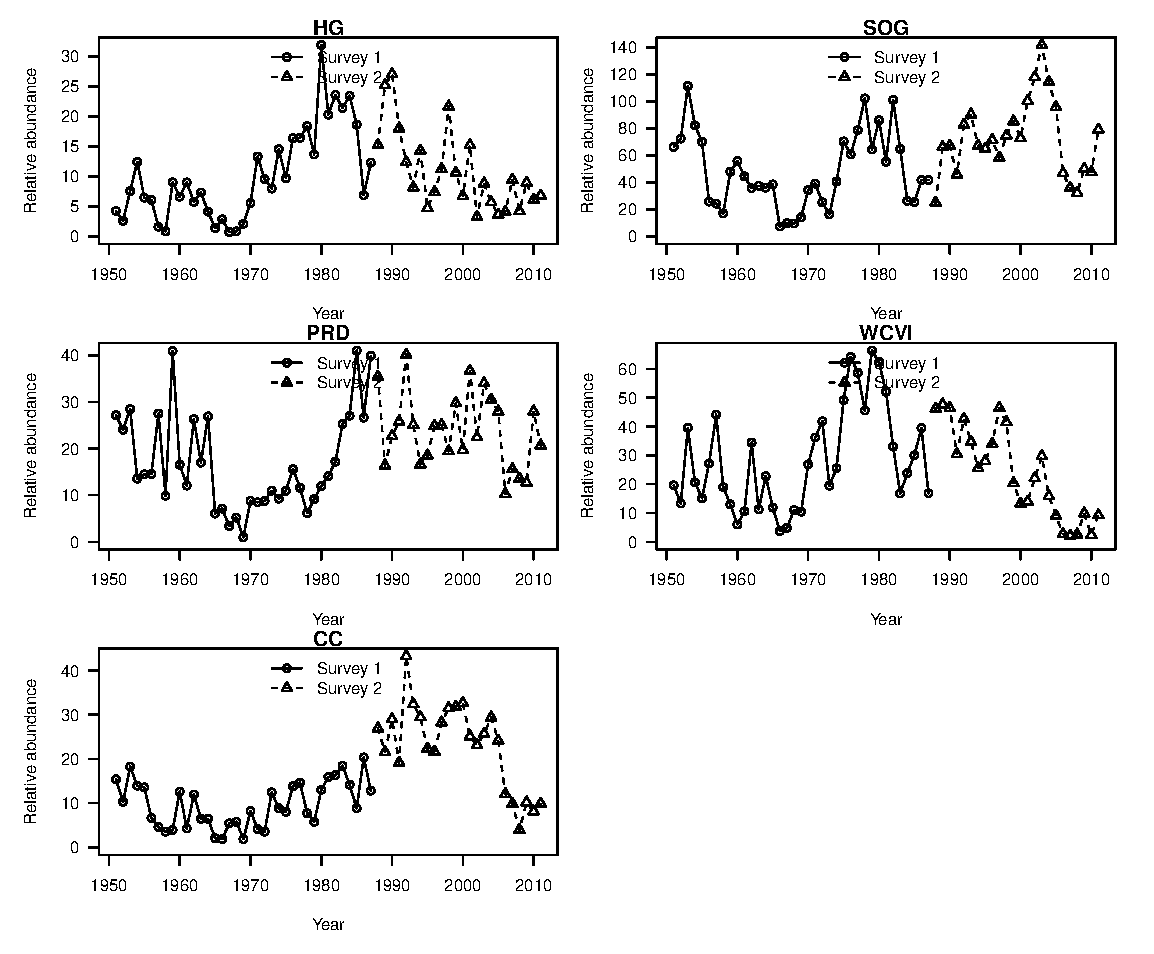
\includegraphics[width=\textwidth]{../Figs/iscam_fig_SurveyMajorAreas.pdf}\\
	\caption{Spawn survey index for Strait of Georgia between 1951 and 2011. The units are actual estimates of spawning biomass (1000s tons), but only the trend information is used in the model fitting.}\label{FigSurvey}
\end{figure}
	
	\subsubsection{Biological samples}
	
	Biological samples are collected from both commercial catch and from the test fishery program.  Commencing  in 1975, test fishery charters supplemented biological samples in areas with poor sampling that was not representative of the stock in that area (i.e., fishing solely on spawning aggregations), or in closed areas. Prior to 2006, test fishing charters were funded through an allocation of fish to the test program; the program is now fully funded by DFO.  Through a contract with DFO, the Herring Conservation and Research Society (HCRS) sub-contracts a number of vessels to collect biological samples.  Industry also conducts pre-season test sets for roe-quality testing in open areas and supplementary biological samples are provided as part of this program.  The following data are collected for all biological samples: fish length, weight, sex, and maturity.  Subsequently these sources of data are combined and information on weight-at-age and proportion-at-age become input data for the stock assessment model.
	
	During the 2010/2011 season a total of XXX biological samples were collected, of which XXX were collected from the test fishery, XXX were collected from the roe fishery, XXX from the food \& bait fishery, XXX from Spawn on Kelp (SOK) operations, and XXX from the summer trawl research survey (Table \ref{XXX}).  Note that the definition of a sample is roughly 100 individual fish.  A summary of biological samples collected from commercial and pre-fishery charters from 2002/03--2010/11 is presented in Table \ref{XXX}).
	
	
	%%Insert Summary of biological samples from the 2010/2011 season here:
	
	%%Insert Summary of biological samples collected and processeed from commercial catch etc. here (Table 2 from Cleary 2011).
	
	\subsubsection{Age composition data}
	
	Ageing data, through the reading of fish scales, are collected from the biological samples taken from the commercial fisheries and test fishery charters. Age composition data is used to determine proportions-at-age and is an essential source of input data to the herring stock assessment model.
	
	Catch-at-age data from the winter seine fishery (top panels of Figures \ref{FigAgeCompsHG}-\ref{FigAgeCompsWCVI}) indicate that this fishery primarily targets younger fish in comparison to the seine-roe and gill net fleets. The winter seine fishery appears not to capture older fish in comparison to the gill net fleet. The shaded polygons in Figures \ref{FigAgeCompsHG}-\ref{FigAgeCompsWCVI} approximates the 95\% distribution of ages in the catch.  Roughly 90\% of the fish landed in the winter seine fishery are younger than age-7, and younger than age-6 in recent years.  In both the winter seine and seine-roe fishery age-2 fish are frequently landed; whereas, age-2 fish are rarely landed in the gill net fisher, and fish to appear to fully recruit to the gear until at least 4-5 years of age.  The mean age of the catch appears to be increasing between 2008 and 2010 in both the gill net and winter seine fishery, and there is no obvious trend in the seine roe fishery.  There is however a declining trend in the older ages caught in the seine-roe fishery since 2006 (erosion of age-structure).

\begin{sidewaysfigure}[!tbp]
	% Requires \usepackage{graphicx}
	\centering
	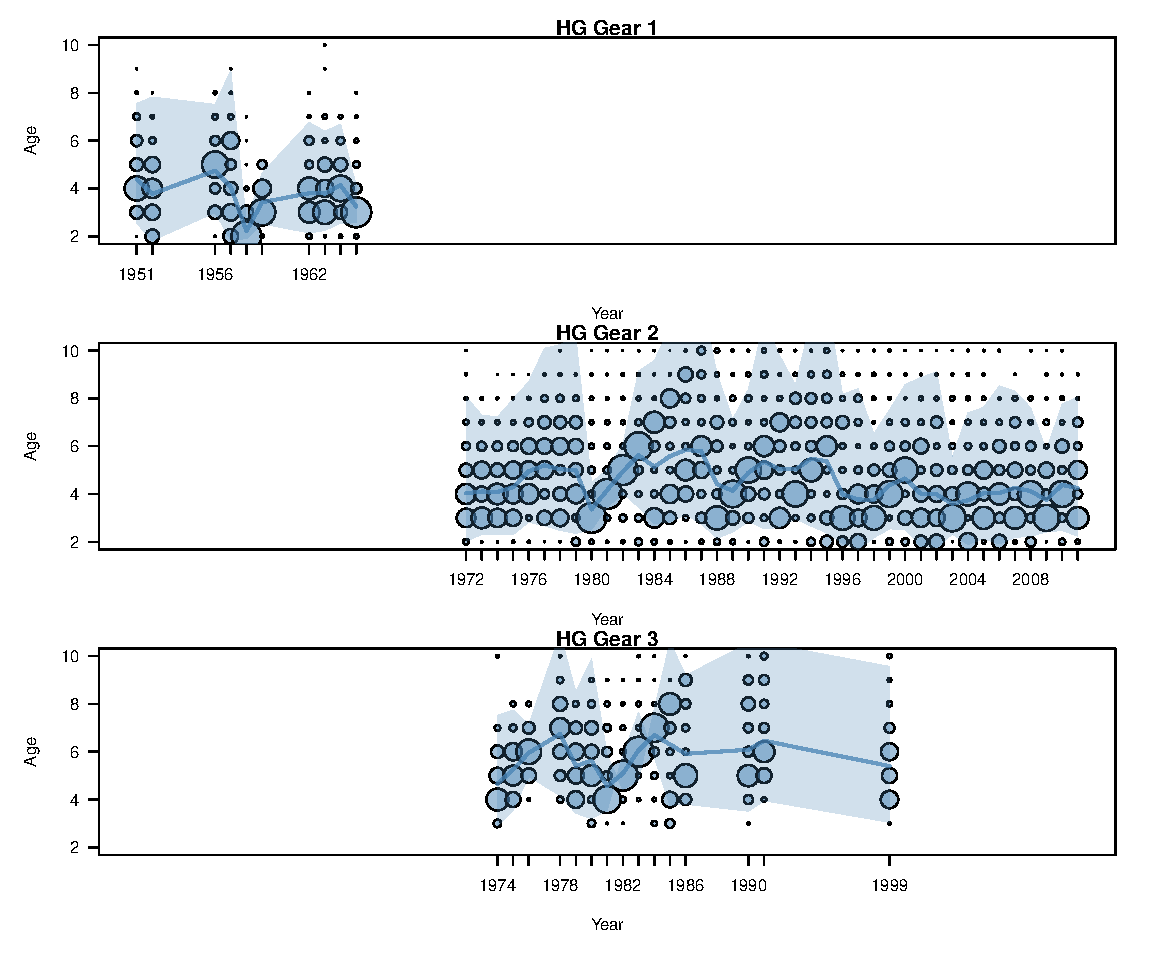
\includegraphics[width=0.85\textwidth]{../Figs/iscam_fig_AgeCompsHG.pdf}\\
	\caption{Bubble plots showing the proportions-at-age versus time for the winter purse seine fishery (top), seine roe fishery (middle) and the gill net fishery (bottom) in Haida Gwaii.  The area of the circle is proportional to cohort abundance, each column sums to 1, zeros are not shown, and age 10 is a plus group. Also shown is the mean age of the catch (line) and the approximate 95\% distribution of ages (shaded polygon) for each year.}\label{FigAgeCompsHG}
\end{sidewaysfigure}

\begin{sidewaysfigure}[!tbp]
	% Requires \usepackage{graphicx}
	\centering
	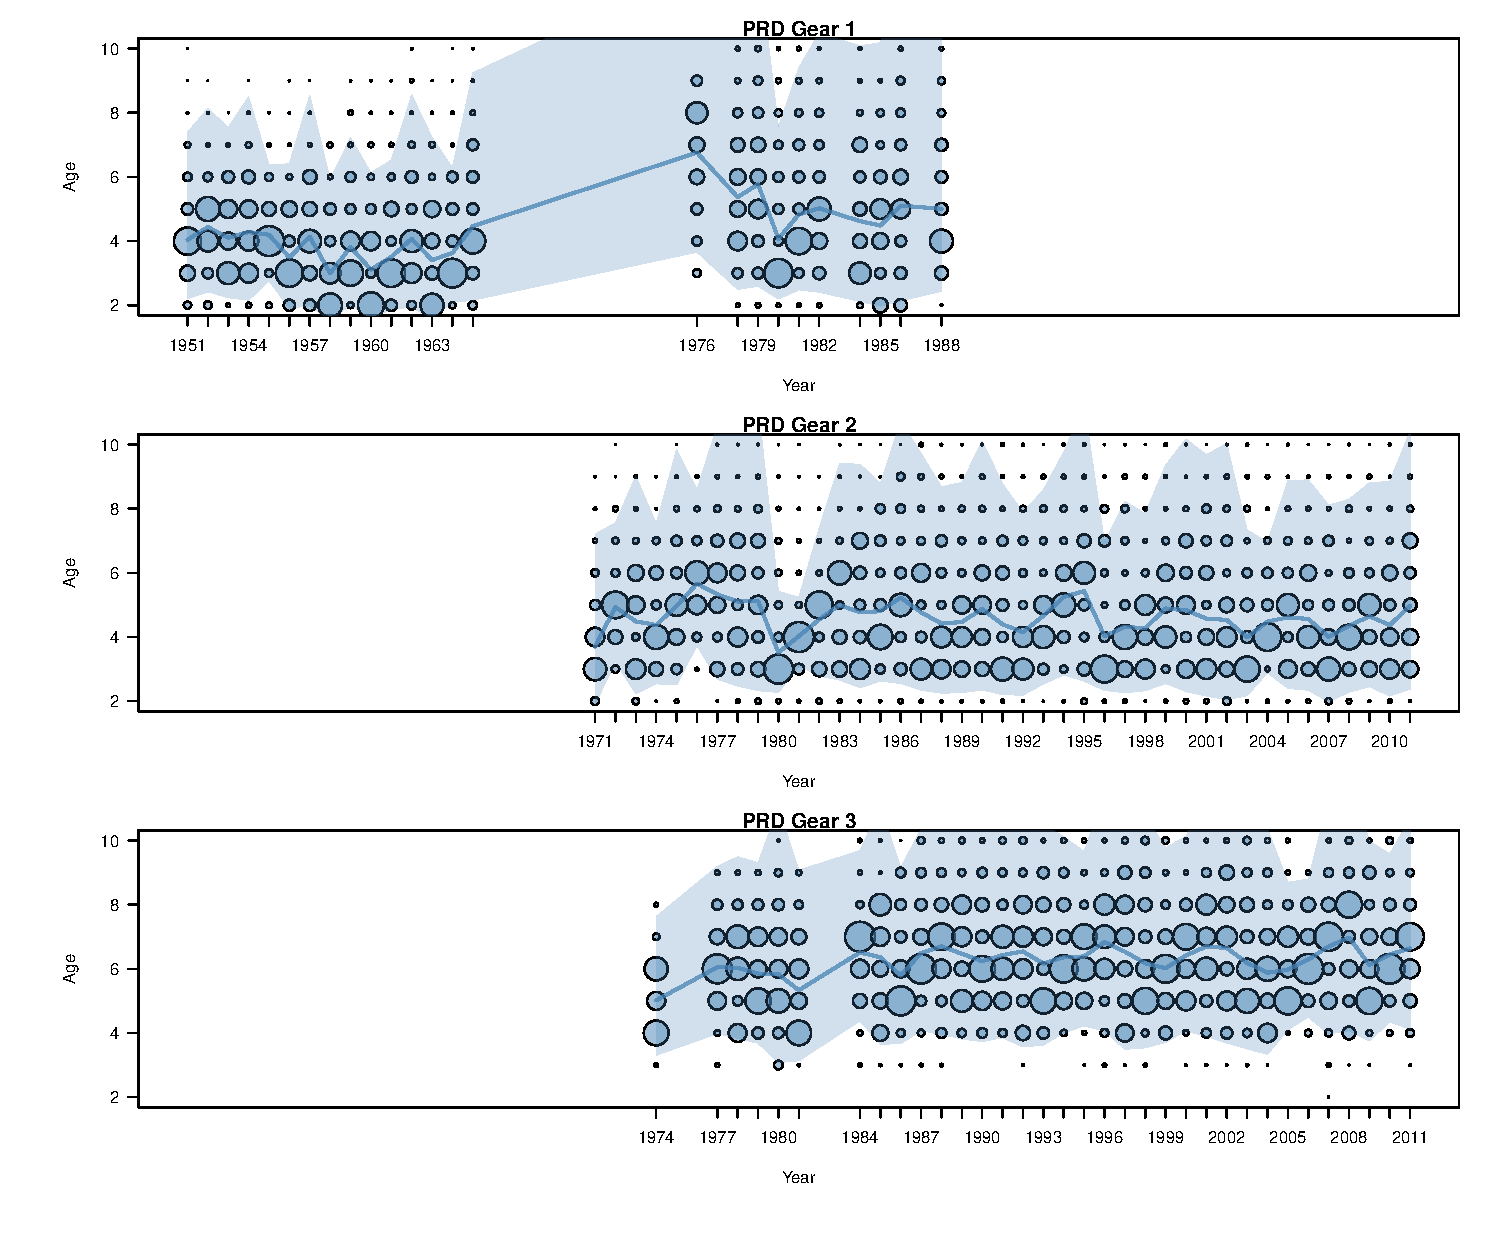
\includegraphics[width=0.85\textwidth]{../Figs/iscam_fig_AgeCompsPRD.pdf}\\
	\caption{Bubble plots showing the proportions-at-age versus time for the winter purse seine fishery (top), seine roe fishery (middle) and the gill net fishery (bottom) in Prince Rupert District.  The area of the circle is proportional to cohort abundance, each column sums to 1, zeros are not shown, and age 10 is a plus group. Also shown is the mean age of the catch (line) and the approximate 95\% distribution of ages (shaded polygon) for each year.}\label{FigAgeCompsPRD}
\end{sidewaysfigure}

\begin{sidewaysfigure}[!tbp]
	% Requires \usepackage{graphicx}
	\centering
	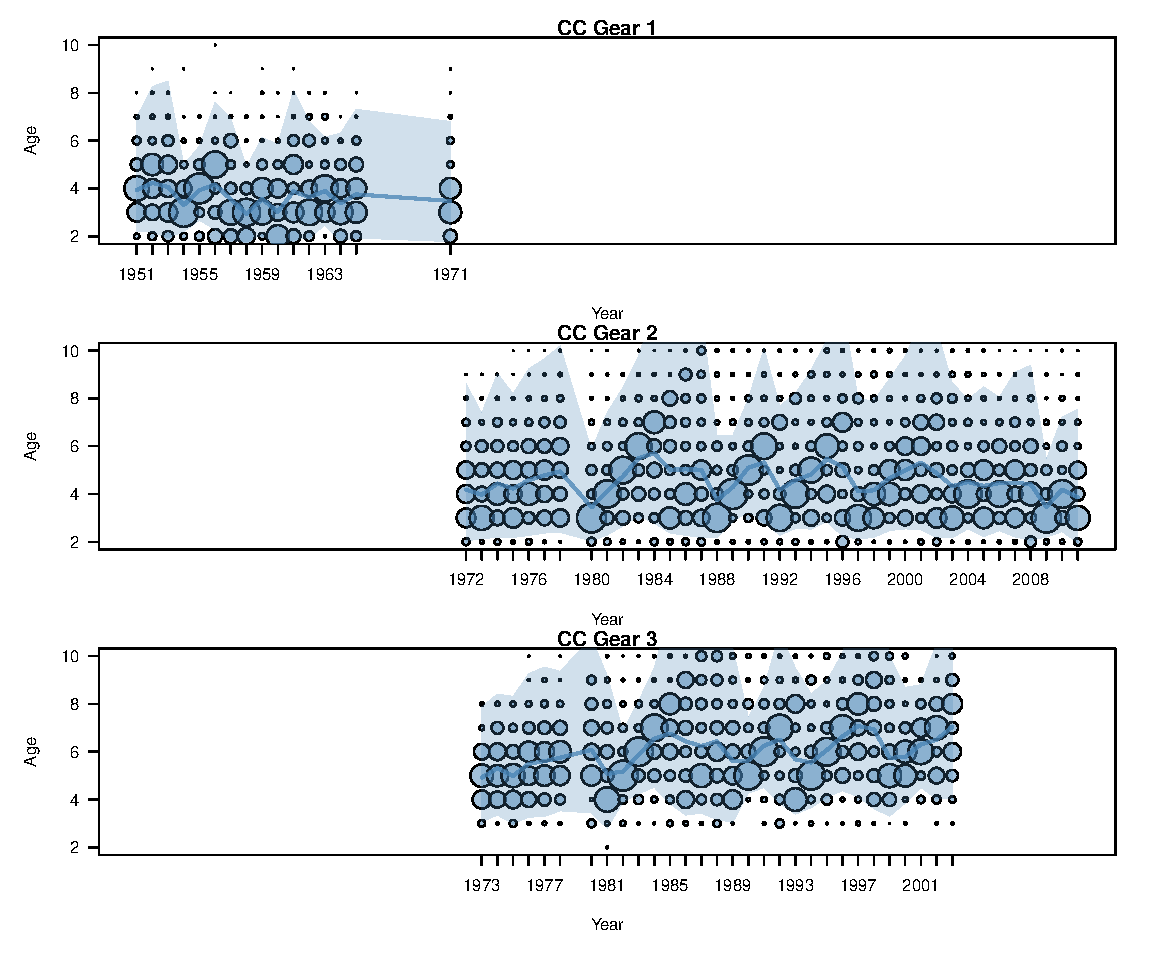
\includegraphics[width=0.85\textwidth]{../Figs/iscam_fig_AgeCompsCC.pdf}\\
	\caption{Bubble plots showing the proportions-at-age versus time for the winter purse seine fishery (top), seine roe fishery (middle) and the gill net fishery (bottom) in the Central Coast region.  The area of the circle is proportional to cohort abundance, each column sums to 1, zeros are not shown, and age 10 is a plus group. Also shown is the mean age of the catch (line) and the approximate 95\% distribution of ages (shaded polygon) for each year.}\label{FigAgeCompsCC}
\end{sidewaysfigure}

\begin{sidewaysfigure}[!tbp]
	% Requires \usepackage{graphicx}
	\centering
	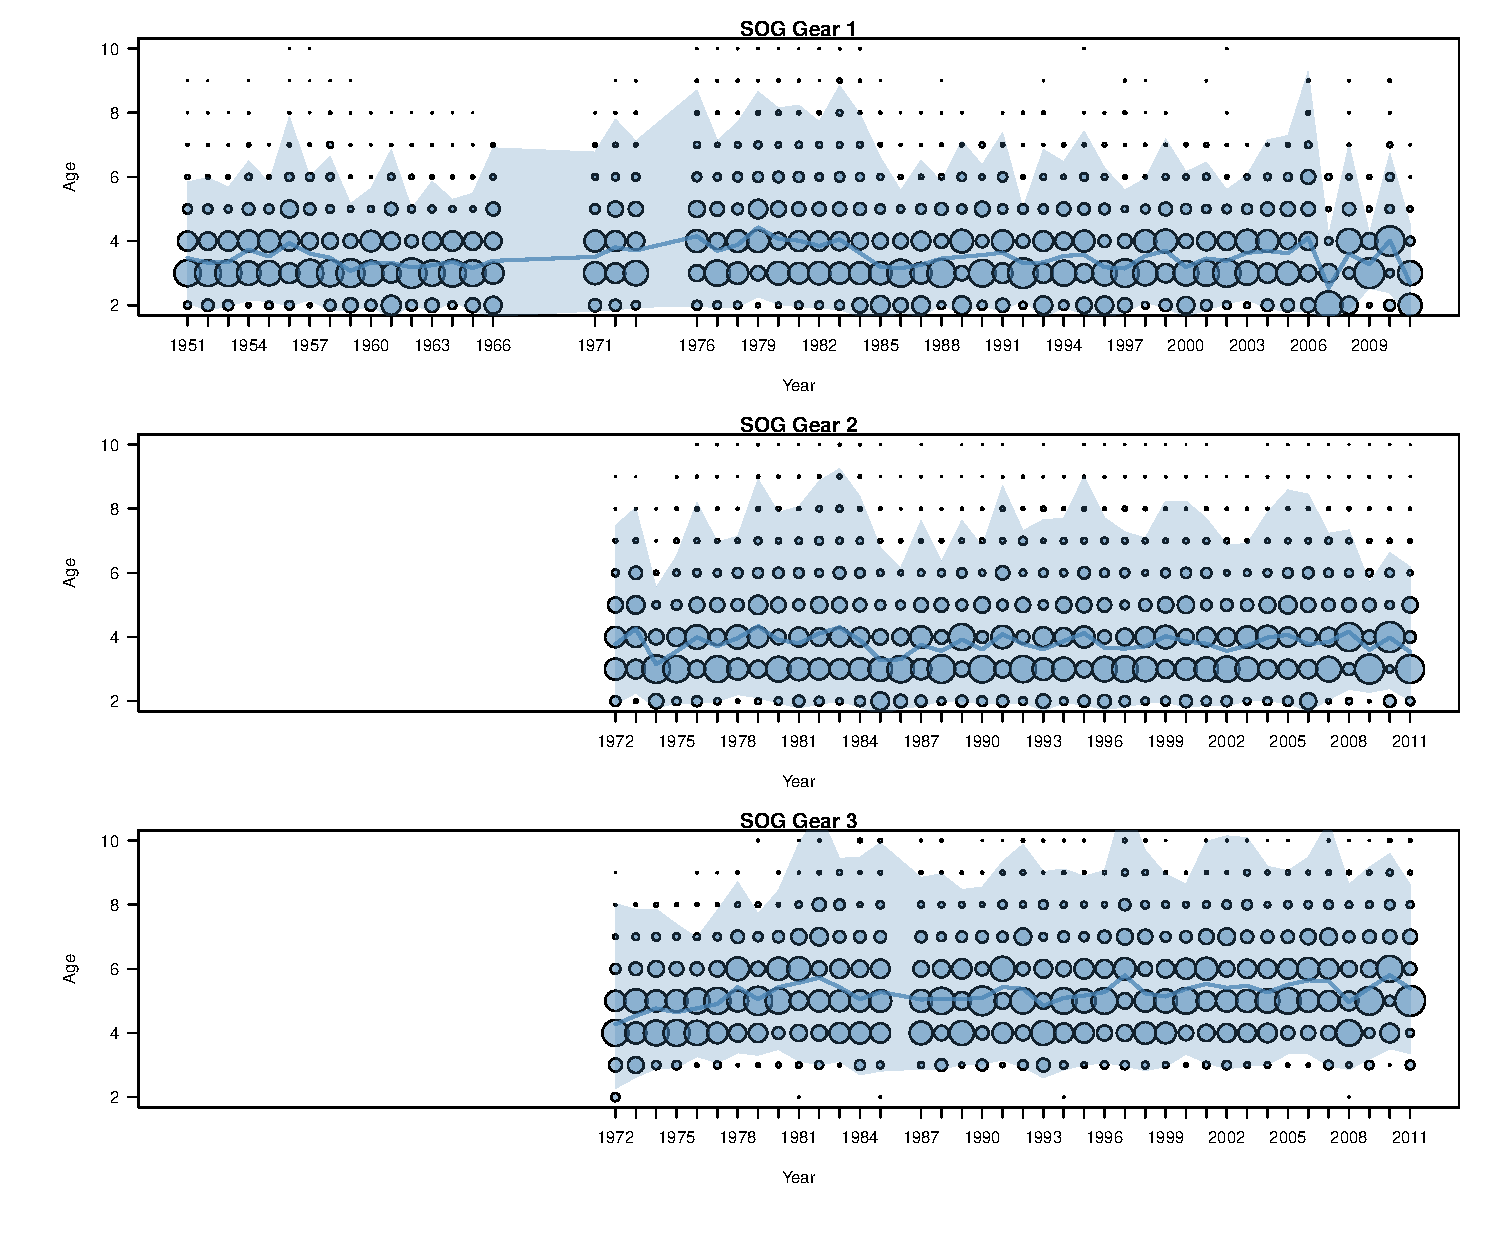
\includegraphics[width=0.85\textwidth]{../Figs/iscam_fig_AgeCompsSOG.pdf}\\
	\caption{Bubble plots showing the proportions-at-age versus time for the winter purse seine fishery (top), seine roe fishery (middle) and the gill net fishery (bottom) in the Strait of Georgia.  The area of the circle is proportional to cohort abundance, each column sums to 1, zeros are not shown, and age 10 is a plus group. Also shown is the mean age of the catch (line) and the approximate 95\% distribution of ages (shaded polygon) for each year.}\label{FigAgeCompsSOG}
\end{sidewaysfigure}

\begin{sidewaysfigure}[!tbp]
	% Requires \usepackage{graphicx}
	\centering
	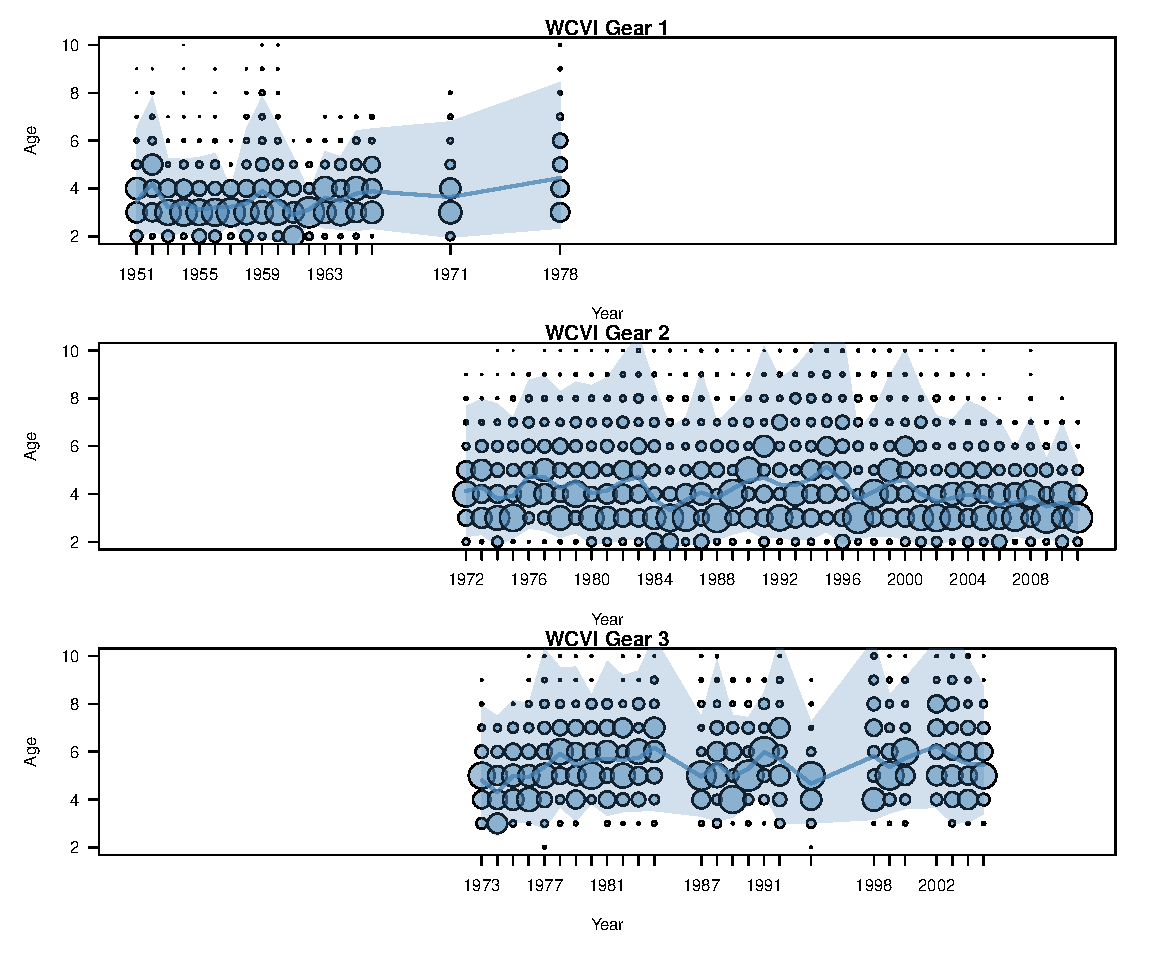
\includegraphics[width=0.85\textwidth]{../Figs/iscam_fig_AgeCompsWCVI.pdf}\\
	\caption{Bubble plots showing the proportions-at-age versus time for the winter purse seine fishery (top), seine roe fishery (middle) and the gill net fishery (bottom) in the West Coast Vancouver Island region.  The area of the circle is proportional to cohort abundance, each column sums to 1, zeros are not shown, and age 10 is a plus group. Also shown is the mean age of the catch (line) and the approximate 95\% distribution of ages (shaded polygon) for each year.}\label{FigAgeCompsWCVI}
\end{sidewaysfigure}





	\subsubsection{Mean weight-at-age data}

	From the mid-1970s until the present, there has been a measurable decline in weight-at-age for all ages in all major stock areas (Figure \ref{FigMeanWt}). Samples collected during the 2009/10 fishing year indicate weights-at-age that are among the lowest on record. This declining weight-at-age may be attributed to any number of factors, including: fishing effects (i.e., gear selectivity), environmental effects (changes in ocean productivity), or it may even be attributed to changes in sampling protocols (shorter time frame over which samples are collected). Declining weight-at-age has been observed in all five of the major stocks, and despite area closures over the last 10-years, has continued to occur in the QCI and WCVI stocks. Although the direct cause of this decline is still to be investigated, this trend has been observed in B.C. and U.S. waters, from California to Alaska \citep{schweigert2002herring}, and merits further research.	The observed mean weight-at-age data appear to have a few erroneous errors that need to be investigated as well; for example, see the apparently small age-10 fish in 2001 in Figure \ref{FigMeanWt}.

\begin{figure}[!tbp]
	% Requires \usepackage{graphicx}
	\centering
	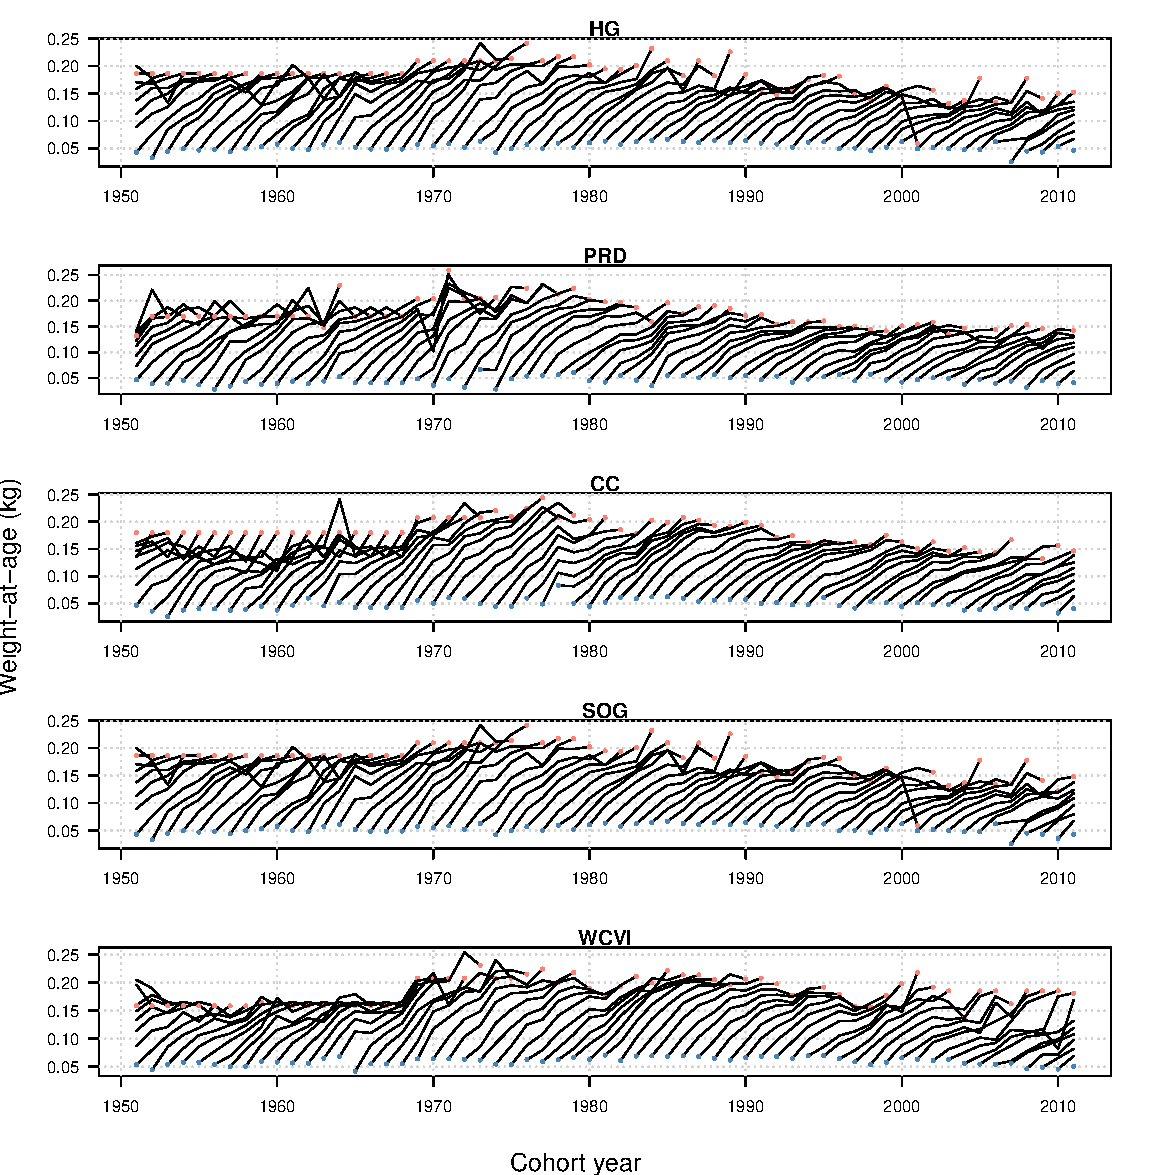
\includegraphics[width=\textwidth]{../Figs/iscam_fig_MeanWt.pdf}\\
	\caption{Empirical mean weight-at-age data by cohort from 1951 to 2011 for ages 2 to 10 in the five major Stock Assessment Regions.}\label{FigMeanWt}
\end{figure}
	

%%%%%%%%%%%%%%%%%%%%%%%%%%%%%%%%%%%%%%%%%%%%%%%%%%%%%%%%%%%%%%%%%%%%%
%%%%%%%%%%%%%%%%%%%%%%%%%%%%%%%%%%%%%%%%%%%%%%%%%%%%%%%%%%%%%%%%%%%%%
%%%%%%%%%%%%%%%%%%%%%%%%%%%%%%%%%%%%%%%%%%%%%%%%%%%%%%%%%%%%%%%%%%%%%	

	\subsection{Analytical methods}
	A new stock assessment platform has been used for the 2011 Pacific herring assessment and this platform is based on the general statistical catch age model first described by \cite{fournier1982general}.  The software platform used is called \iscam, which stands for integrated Statistical Catch Age Model.  The source code and documentation for \iscam\ is freely available from \url{https://sites.google.com/site/iscamproject/}, or from a subversion repository at \url{http://code.google.com/p/iscam-project/}.  Ideally, the results of this report could easily be repeated just by downloading the necessary software and using the data and control files presented in the appendix of this paper. A complete technical description of \iscam\ is provided in Appendix \ref{appiSCAM}.
	
	In short, for each stock a two input files are required for \iscam: (1) a data file that contains the historical catch, survey, life-history and age-composition information, and (2) a control file that specifies initial parameter values, priors, selectivity options, and various other controls that specify options for time-varying natural mortality, type of recruitment model, etc.  Each major and minor stock has its own data and control file and these are provided in Appendix \ref{AppendixDataFiles} such that these results can be verified by an independent reviewer using the \iscam\ software.
	
	Estimated model parameters includes the initial numbers-at-age, annual age-2 recruits, annual fishing mortality rates for each gear, selectivity parameters, natural mortality rates, parameters that describe the observation error and process error variance, and the unfished age-2 recruits and the steepness of the stock recruitment relationship.  The total number of estimated parameters differs for each stock assessment region depending on the number of years of active fishing, assumptions about selectivity, and the number of assumed nodes in natural mortality rates.  In general the total number of estimated parameters ranges from  

	
	\subsection{Simulation testing}
	
		The purpose of conducting simulation testing is two fold: (1) to demonstrate that the model is capable of estimating model parameters given perfect information, and (2) to examine precision and bias in parameter estimates (and corresponding management quantities) in the presence of observation and process errors.  To conduct simulation testing using \iscam, the following command line option \verb"-sim 1234" is used, where 1234 is a unique random number seed.  There is also a special seed number \verb"-sim 000" that generates data with no error.  That is the simulation model is deterministic, the relative abundance data are directly proportional with 0 observation error, and the age-composition data is exactly replicates the true vulnerable proportions-at-age.  The model is conditioned on the historical catch data specified in the data file, and the true parameter values used to simulate the data are those that are specified in the control file.

	
		\subsubsection{Estimation performance with perfect information}
		 
When simulating data with perfect information, there are a couple of things that need to be highlighted here when trying to estimate parameters from data that contain no error.  First, the phases for the precision and variance partitioning parameters ($\vartheta$ and $\rho$) should be set to a negative number.  There are no error in the data, therefore, there is no need to estimate the variance terms for the error distributions.  Second, in the control file, the initial value for the precision ($\vartheta$) should be set to an extremely large number (e.g., 4999.999, assuming the upper bound is 5000).  The reason to set this number large is to minimize the slight bias due to the lognormal bias correction in the stock recruitment relationship (i.e., the $-0.5\tau^2$ term in \ref{T4.12}, or \ref{T4.13}). The control file used to simulate the fake data is provided in Table \ref{TableSOGsimCtrl}.




		
		\subsubsection{Bias \& precision with observation \& process errors}
To determine bias and precision of parameter estimates when the model is confronted with both observation error and process error, a series of Monte Carlo trials are performed and $\log_2$ ratios are used to measure the distribution of estimated parameters ($\acute{\theta}$) from the true value($\theta$).  The log2 ratio
\[ \log_2\left(\frac{\acute{\theta}}{\theta}\right) \] is zero when $\acute{\theta}=\theta$, is 1 when $2\acute{\theta}=\theta$, and is -1 when $0.5\acute{\theta}=\theta$.  Box plots are used to examine the distribution of 50 trials where a unique random number seed is used for each trial.  For the purposes of the simulation experiments only, we assume that the proportion of the total variance associated with observation error is known ($\rho = 0.25$) and estimate the total variance.  The total precision is set to 2.50 which is equivalent to a total standard deviation of 0.4.  The control file used for the Monte Carlo procedures is provided in Table \ref{TabelSOGmcCTRL}.


%% ================================================================ %%
\subsection{Comparison of HCAM with \iscam}\label{secMethodsHCAM}
	
	There are a number of different statistical assumptions and structural differences between the previous assessments using HCAM (Herring Catch Age Model) and \iscam.	  Here I briefly summarize the differences and similarities between the two approaches, and we first attempt to formulate the \iscam\ model to be as similar as possible to the last implementation of HCAM used in \cite{Clear2010}.
	
	The objective function in the HCAM model has four major components to it: 1) the likelihood of the age composition data, 2) the likelihood of the commercial catch data, 3) the likelihood of the spawn data, and 4) the prior densities for estimated model parameters.  In the following subsections are more detailed descriptions of how the \iscam\ model was set up to best approximate the HCAM implementation.
	
	For the GN fishery, HCAM implements a time varying selectivity scheme as a function of the average weight-at-age.  At present this is not implemented in \iscam, and after a day of investigation I (SJDM) was not able to come up with a feasible solution to make the models more comparable. Alternative options for changes in selectivity will be investigated further later in this paper.
	
	
\subsubsection{Age-composition data}
There are two alternative likelihoods specified for the age-composition data in the HCAM model \citep[see Table 8 in Appendix B in][]{Clear2010}.  It is unclear which likelihood is actually used, the multinomial likelihood (T8.1), or the robust normal approximation (T8.2), or both in the  assessment.  In any event, \iscam\ implements a multivariate logistic negative log-likelihood for age-composition data (see equation \ref{eq8} above), with the intention of weighting these data based on the conditional maximum likelihood estimate of the variance.  In addition, we require a minimum observed proportion of at least 1\% in each age class, in years and ages where the observed proportion is less than 1\% the consecutive ages grouped into a single age-class which reduces the effective number of age-classes (this is some what analogous to a plus group).

\subsubsection{Commercial catch data}
	In the HCAM assessment, commercial catch was assumed to be know with a high degree of certainty; observation errors were assumed lognormal, and the standard deviation specified in the code is fixed at 0.0707 (variance of 0.005) for all three periods.  The analogous setup in \iscam\ is to fix the assumed standard deviation for the catches in the last phase to 0.0707.
	
\subsubsection{Spawn survey data}
 	For the Strait of Georgia spawn survey, the assumed standard deviations in HCAM were specified at 0.35 and 0.3 for the pre and post 1988 periods.  To carry out the same assumptions in \iscam\ the relative weights for the pre and post 1988 survey data were fixed at 1.0 and 1.1666, respectively.  In \iscam\ the total error (or precision=1/variance) is estimated and partitioned into components of observation error (spawn survey residuals) and process error (recruitment deviations).  To implement the same observation error and process errors in the \iscam\ model (standard deviations of 0.35 and 0.8, respectively for observation errors and process errors in HCAM) the total precision was fixed at $\vartheta=1/1.15$, and the proportion assigned to observation error was fixed at $\rho = 0.35/1.15$.

\subsubsection{Specification of prior distributions}
	Starting with the prior density for natural mortality in HCAM, the average natural mortality rate is assumed to be normal with a mean of 0.45, and a standard deviation of 0.2 \citep[see Table 3 in][]{Clear2010}.  The average natural mortality rate in \iscam\ is estimated in the log scale; using a normal prior for the $\ln(M)$ is equivalent to a lognormal prior for $M$.  A lognormal prior is appropriate for this parameter as natural mortality rates must be positive; however, there is no equivalent analytical transformation to the normal distribution that was used in the HCAM assessment.  Here we have specified a  normal prior for $\ln(M)$ with a log mean of $\ln(0.45)=-0.7985$ and a log standard deviation of 0.4 to approximate the variance specified in the normal distribution used in the previous HCAM assessment.
	
	The base HCAM model also allows for a random walk in natural mortality rate implemented as:
\[
M_t =\begin{cases}
	 \psi, \quad t=t'\\
	 M_{t-1}\exp(d_t^M), t>t'
	 \end{cases}
\]
where $d_t^M$ are annual natural mortality deviations that are assumed to be normally distributed with a mean 0 and a standard deviation of 0.10, and $\psi$ is an estimated initial value for natural mortality.  The implementation of time varying natural mortality is similar in \iscam\ in that it is a random walk process, but the components of the objective function include a prior for the initial value of $M$ (as specified in the previous paragraph) and that the first differences between natural mortality deviations are normally distributed. Again, this structure allows natural mortality rates to drift away from central tendency and long-term changes in $M$ could have profound effects on reference point calculations.  For the comparison with the HCAM model, the first differences in annual natural mortality deviations were assumed to have a mean 0 and a standard deviation of 0.10.

Annual recruitment deviations in the HCAM implementation were assumed to be normally distributed on a log scale with a mean of zero and a standard deviation of 0.8.  To set up an equivalent assumption in \iscam, the total variance ($\vartheta$) and ratio of the total variance ($\rho$) that explains observation error in the spawn survey must be specified \emph{a priori}. In the HCAM model the variance terms for the observation errors and process errors are not estimated and assumed to be known; the standard deviation for recruitment variation was set at 0.8 and the standard deviation for observation errors in the spawn survey was fixed at 0.35 and 0.3 for the pre and post 1988 data, respectively.  These variance terms can be estimated within the \iscam\ model, or treated as fixed constants; however, \iscam\ estimates the total error and partitions the variance into observation ($\sigma^2$) and process error ($\tau^2$) components.  To make the same assumptions about the variance terms in \iscam\ as those that were used in HCAM the following values were used $\vartheta=1/1.15=0.8695652$, and $\rho=0.3043478$, and the weights assigned to the post 1988 spawn data were set at 1.1666 and 1.0 for the pre 1988 spawn data.

The prior for steepness in the HCAM model was based on a lognormal distribution with a logmean of 0.67 and a standard deviation of 0.17.  For the Beverton-Holt stock recruitment model, steepness must lie in the interval of  $0.2<h\leq1.0$; a Beta distribution is an appropriate density function for this parameter. In the \iscam\ implementation, a Beta distribution is used and to approximate the distribution used in the HCAM model, the shape and rate parameters specified are 10.0 and 4.925373, respectively.  These values corresponds to a mean of 0.67 and a standard deviation of 0.1178 for the Beta prior.

The last informative prior that is not explicit in the table of priors in the HCAM model is the scaling parameter ($q$) for the spawn survey.  The spawn survey data are broken into two separate time series, pre and post 1988 when the survey switch from from a surface estimate to dive surveys for estimating total egg deposition.  In the HCAM implementation, a very informative prior for $q$ in the post 1988 period was used where the mean was fixed at $q=1.0$ and not permitted to vary (i.e., $\sigma_q=0$).  The scaling parameter in the first period was then freely estimated. Again, to emulate these assumptions in the \iscam\ implementation a normal prior for $\ln(q)$ with a mean =0 and a standard deviation of 0.001 was used for the post 1988 data and a uniform prior for the pre 1988 data.

		
	\subsection{Retrospective analysis}
	A retrospective analysis was conducted for each of the major and minor SARs.  The retrospective analysis successively removes the last 10-years of data and examines changes in estimates of spawning biomass and estimated reference points.  
	
	\subsection{Abundance and recruitment forecasts}
	The abundance forecast for the upcoming fishing season, also referred to as pre-fishery biomass, is defined as the predicted biomass of age-4 fish and older plus the number of age-3 fish recruiting in year $T+1$.  The abundance estimates are based on the median values from the sampled posterior distribution.  Age-3 recruits are based on poor, average, and good recruitment scenarios; see next paragraph for definitions of poor, average and good.
	
	The recruitment forecasts are based on the surviving number of age-3 fish at the start of the fishing season times the average weight-at-age 3 in the last 5 years. The definitions of poor, average, and good recruitment are as follows: \textbf{Poor} is the average recruitment from the 0-33 percentile, \textbf{Average} is the average recruitment from the 33-66 percentile, and \textbf{Good} is the average recruitment from the 66-100 percentile.  Note that all cohorts from 1951 to 2010  were included in the recruitment forecast calculation.	

	
	
